\documentclass[11pt,spanish,dvipsnames]{article}
\usepackage[utf8]{inputenc}
\usepackage{babel}
\usepackage{fullpage}
\usepackage{listings}
\usepackage{mathpazo}
\usepackage{enumitem}
\usepackage{courier}
\usepackage{xcolor}
\usepackage{textcomp}
\usepackage{amsmath}
\usepackage{amssymb}
\usepackage{tikz}
\usepackage{fancyhdr}
\usepackage{graphics}
\usepackage{array}

\newcommand{\titulo}{Certamen 1 [SJ, v1], miércoles 19 de diciembre de 2011}
\newcommand{\cc}[1]{\hfil\texttt{#1}\hfil}
\newcommand{\pond}[1]{[{\small\textbf{#1\%}}]}

\pagestyle{fancy}
\lhead{%
  {\Large\bfseries Programación---\titulo} \\
  Nombre: \nombre\hfill
  Rol:    \rol
  \vspace{2ex}
}
\chead{}\rhead{}\lfoot{}\cfoot{}\rfoot{}
\renewcommand{\headrulewidth}{0pt}
\addtolength{\headheight}{7ex}
\headsep=4ex


\newcommand{\onelinerule}{\rule[2.3ex]{0pt}{0pt}}
\newcommand{\twolinerule}{\rule[6.2ex]{0pt}{0pt}}
\newcommand{\respuesta}{\framebox[\textwidth]{\twolinerule}}
\newcommand{\nombre}{%
  \begin{tikzpicture}[xscale=.4,yscale=.7]
    \draw (0, 0) rectangle (22, 1);
  \end{tikzpicture}%
}
%\newcommand{\rol}   {\framebox[0.3\textwidth]{\onelinerule}}
\newcommand{\rol}{%
  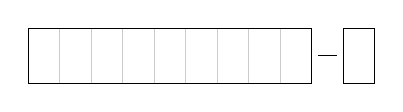
\begin{tikzpicture}[xscale=.4,yscale=.7]
    \draw[gray!40] ( 0, 0) grid      ( 9, 1);
    \draw          ( 0, 0) rectangle ( 9, 1);
    \draw          (10, 0) rectangle (11, 1);
    \draw (9 + .2, .5) -- (10 - .2, .5);
  \end{tikzpicture}%
}
\newcommand{\li}{\lstinline}
\providecommand{\pond}[1]{[{\small\textbf{#1\%}}]}

\lstdefinelanguage{py}{%
  classoffset=0,%
    morekeywords={%
      False,class,finally,is,return,None,continue,for,lambda,try,%
      True,def,from,nonlocal,while,and,del,global,not,with,print,%
      as,elif,if,or,yield,assert,else,import,pass,break,except,in,raise},%
    keywordstyle=\color{black!80}\bfseries,%
  classoffset=1,
    morekeywords={int,float,str,abs,len,raw_input,exit,range,min,max,%
      set,dict,tuple,list,bool,complex,round,sum,all,any,zip,map,filter,%
      sorted,reversed,dir,file,frozenset,open,%
      array,zeros,ones,arange,linspace,eye,diag,dot},
    keywordstyle=\color{black!50}\bfseries,%
  classoffset=0,%
  sensitive=true,%
  morecomment=[l]\#,%
  morestring=[b]',%
  morestring=[b]",%
  stringstyle=\em,%
}

\lstdefinelanguage{testcase}{%
  moredelim=[is][\bfseries]{`}{`},%
  backgroundcolor=\color{gray!20},%
}

\lstdefinelanguage{file}{%
  frame=single,%
}

\lstset{language=py}
\lstset{basicstyle=\ttfamily}
\lstset{columns=fixed}
\lstset{upquote=true}
\lstset{showstringspaces=false}
\lstset{rangeprefix=\#\ }
\lstset{includerangemarker=false}

\newlist{certamen}{enumerate}{1}
\setlist[certamen]{%
  label=\arabic*.,
  font=\LARGE\bfseries,%
  labelindent=-.5in,%
  leftmargin=0pt,%
  labelsep=1em%
}



\begin{document}

  \begin{enumerate}[font=\Large\bfseries]

    % Entender programas
    \item%[1a.]
      \pond{25}
      Indique qué es lo que imprimen los siguientes programas.

      \foreach \x in {1,2} {
        \noindent
        \begin{minipage}[b]{.5\textwidth}
          \lstinputlisting{p\x.py}
          \framebox[.8\textwidth]{\rule[10ex]{0pt}{0pt}}
          \vspace{0.4em}
        \end{minipage}
      }

    %\item[1b.]
      Rutee el siguiente programa
      e indique qué es lo que imprime.

      Cada vez que el valor de una variable cambie,
      ponga su valor en una nueva fila de la tabla.
      La tabla tiene filas de sobra.

      \begin{minipage}[T]{.5\textwidth}
        \lstinputlisting{ruteo.py}
        \framebox[.8\textwidth]{\rule[10ex]{0pt}{0pt}}
      \end{minipage}
      \begin{minipage}[t]{.4\textwidth}\centering
        \begin{tabular}{|*{3}{p{2.6em}|}}\hline
            \cc{i} & \cc{j} & \cc{g} \\ \hline\hline
            && \\\hline && \\\hline && \\\hline && \\\hline && \\\hline
            && \\\hline && \\\hline && \\\hline && \\\hline && \\\hline
            && \\\hline && \\\hline && \\\hline && \\\hline && \\\hline
            && \\\hline && \\\hline && \\\hline && \\\hline && \\\hline
            && \\\hline && \\\hline && \\\hline && \\\hline && \\\hline
         \end{tabular}
      \end{minipage}

    \newpage
    \item %
      \def\rPlaza{47}
      \def\rExtVerde{35}
      \def\rIntVerde{20}
      \def\rPileta{7}
      \tikzstyle{cemento}=[fill=black!50]
      \tikzstyle{pileta}=[fill=black!80]
      \tikzstyle{verde}=[fill=Green]
      \tikzstyle{gente}=[fill=Yellow]
      \pond{25}
      Para celebrar el aniversario de la fundación de Kreisdorf,
      la alcaldesa ha organizado un espectáculo aéreo,
      que finalizará con el aterrizaje de un paracaidista
      en la plaza del pueblo.

      \begin{minipage}[T]{.6\textwidth}
        La plaza es circular, y su radio es de \rPlaza{} metros.
        En su centro hay una pileta
        (\tikz\filldraw[pileta] (0, 0) circle (.6ex) ;)
        de \rPileta{} metros de radio.
        Además, hay cuatro áreas verdes
        (\tikz\filldraw[verde]
              ( 67 :       1.0ex) arc
              ( 67 : 112 : 1.0ex) --
              (      112 : 2.1ex) arc
              (112 :  67 : 2.1ex) -- cycle ;),
        en las posiciones indicadas en la figura;
        los radios interno y externo de las áreas verdes
        son, respectivamente, \rIntVerde{} y \rExtVerde{} metros.
        El resto de la superficie es cemento.
        \\[.6ex]
        El público que irá a presenciar el espectáculo
        se ubicará en el sector de la plaza
        indicado en la figura
        (\tikz\filldraw[gente]
              (0, 0) -- (0:3ex) arc (0:30:3ex) -- cycle;).
        \\[.6ex]
        El paracaidista ha encargado el desarrollo de un programa
        que le permita planificar su trayectoria
        para evitar caer en un lugar peligroso.
        El punto de aterrizaje
        está definido por dos valores:
        su distancia al centro de la plaza
        y el ángulo con respecto a las coordenadas indicadas en la figura.

      \end{minipage}
      \hfill
      \begin{minipage}[T]{.3\textwidth}
        \begin{tikzpicture}[scale=.046]
          % plaza
          \filldraw[cemento] (0, 0) circle (\rPlaza);

          % lineas y ángulos
          \tikzstyle{lineas}=[dashed, gray!50, thick]
          \foreach\angulo in {0,45,...,315} {
            \draw[lineas] (0, 0) -- (\angulo : \rPlaza);
            \node[font=\tiny] at (\angulo: 52) {\angulo\(^{\circ}\)};
          }
          \draw[lineas] (0, 0) circle (\rExtVerde);
          \draw[lineas] (0, 0) circle (\rIntVerde);

          % gente
          \filldraw[gente] (0, 0) -- (45 : \rPlaza) arc (45 : 90 : \rPlaza) -- cycle;

          % pileta
          \filldraw[pileta] (0, 0) circle (\rPileta);

          % areas verdes
          \foreach\i in {0,2,4,6} {
            \filldraw[verde]
              ({\i * 45} :                   \rIntVerde) arc
              ({\i * 45} : {(\i + 1) * 45} : \rIntVerde) --
              (            {(\i + 1) * 45} : \rExtVerde) arc
              ({(\i + 1) * 45} : {\i * 45} : \rExtVerde) -- cycle;
          }

          % distancias
          \foreach\dist in {\rPlaza,\rExtVerde,\rIntVerde, \rPileta} {
            \node[font=\tiny] at (247: \dist) {\dist};
          }

        \end{tikzpicture}
      \end{minipage}

      Escriba un programa que,
      a partir de la distancia y el ángulo de aterrizaje,
      le indique al paracaidista donde caerá.
      El programa debe imprimir
      \li!PILETA!, \li!AREA VERDE!, \li!PUBLICO!, \li!CEMENTO! o \li!FUERA DE LA PLAZA!.

      \begin{minipage}[t]{.26\textwidth}
        \lstinputlisting[language=testcase,frame=single,linerange=CASO\ 1-FIN\ CASO\ 1]{casos-paracaidista.txt}
      \end{minipage}
      \hfill
      \begin{minipage}[t]{.26\textwidth}
        \lstinputlisting[language=testcase,frame=single,linerange=CASO\ 2-FIN\ CASO\ 2]{casos-paracaidista.txt}
      \end{minipage}
      \hfill
      \begin{minipage}[t]{.26\textwidth}
        \lstinputlisting[language=testcase,frame=single,linerange=CASO\ 3-FIN\ CASO\ 3]{casos-paracaidista.txt}
      \end{minipage}

    \newpage
    \item
      \pond{25}
      En el idioma de la tribu de los Stringones,
      la mayoría de las palabras tienen muchas letras
      que se repiten de manera consecutiva.

      El sabio de la tribu ideó un sistema
      para escribir las palabras de manera abreviada:
      cada letra aparece antecedida de un número,
      indicando cuántas veces está repetida.
      Por ejemplo, la palabra \li!pppprrrrrogggrraaa!
      se abrevia \li!4p5r1o3g2r3a!.

      Desarrolle un programa
      que reciba como entrada una palabra abreviada,
      y entregue como salida la palabra original.
      Suponga que ninguna letra
      aparece más de nueve veces seguidas.

    \newpage
    \item
      \pond{25}
      El \emph{enrachao} es un juego muy popular
      entre los niños de la aldea de Pythonia.

      El juego consiste en lanzar varias veces un dado.
      Apenas aparece el número 1, el jugador pierde.
      Para ganar, a un jugador debe aparecerle un número
      (distinto de 1)
      tantas veces consecutivas como indica el mismo número
      (por ejemplo, el 5 cinco veces seguidas).

      Escriba un programa que reciba como entrada
      todos los números obtenidos al lanzar el dado
      hasta que termine el juego,
      y le indique al usuario si ganó o perdió.

      \begin{minipage}[t]{.26\textwidth}
        \lstinputlisting[language=testcase,frame=single,linerange=CASO\ 1-FIN\ CASO\ 1]{casos-enrachao.txt}
      \end{minipage}
      \hspace{1em}
      \begin{minipage}[t]{.26\textwidth}
        \lstinputlisting[language=testcase,frame=single,linerange=CASO\ 2-FIN\ CASO\ 2]{casos-enrachao.txt}
      \end{minipage}

  \end{enumerate}
\end{document}

